%\paragraph{Biological process}
The stringent response is a fundamental regulation of the bacteria that regulates its growth rate and acts on practical all aspects of the cell. Discovered when amino-acid starving a bacteria (stringent response) compared to a rich nutriment response (relaxed response), the bacteria produces alarmones (p)ppGpp that induces the stringent response. Now stringent response means any response linked to the presence of the alarmones, including other stresses than the amino-acid starvation. The stringent response is different between {\it Escherichia Coli} and {\it Bacillus Subtilis} in its mechanism. The following text is principally based on the reviews of \citet{kriel_direct_2012} and of \citet{wolz_synthesis_2010}.

%\medskip

\paragraph{Alarmones synthesis / hydrolysis}
Figure \ref{tab:compareColiSubAlarmoneProd} summarizes the current knowledge.
\begin{figure}[hbtp]
  \centering
  % Requires \usepackage{graphicx}
  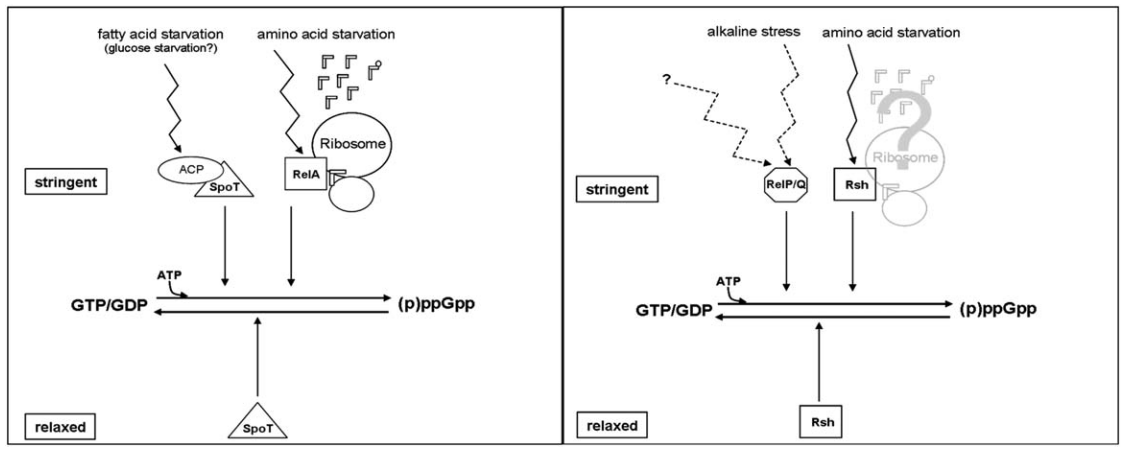
\includegraphics[width=15cm]{figure/alarmoneProd.png}\\
  \caption{Comparison of alarmones synthesis and hydrolysis between Escherichia Coli (left) and Bacillus Subtilis (right) \citep{wolz_synthesis_2010}}\label{tab:compareColiSubAlarmoneProd}
\end{figure}
Rsh (which is also referred to as RelA) in {\it B. Subtilis} and SpoT in {\it E. Coli} are bifunctional (the others being monofunctional) enzymes that can perform synthesis and hydrolysis. They have two conformations ((p)ppGpp-hydrolase-OFF/(p)ppGpp-synthase-ON and hydrolase-ON/synthase-OFF) that is regulated by the C-terminal domain as its truncation enhances the synthase activity. It is not known if, as in the case of {\it E. Coli}, Rsh binds to a ribosome to sense the amino-acid starvation and more precisely the presence of uncharged tRNA. In {\it E. Coli}, RelA binds to a ribosome and is thought to unbind in the presence of an uncharged tRNA in the A-site. This unbinding activates the synthetase function of RelA and inhibits the rebinding during a period of time. In {\it B. Subtilis}, it is knwon that there are only one bifunctional enzyme (Rsh) and only two monofunctional ones (RelP seems to be connected to competence and is encoded by yjbM whereas RelQ seems to be connected to persistence and virulence and is encoded by ywaC) that lack the \ce{Mn^2+}-dependent hydrolase domain \citep{GaL:15}.

%\medskip

\paragraph{Overall effect of alarmones}
It is estimated that, in exponential gorwth conditions, the concentration of alarmones is less than 20 pmol per optical-density unit by rises to millimolar levels in response to adverse growth conditions, such as amino acid starvation \citep{ababneh_rela_2015}. The effect of the alarmones on proteobacteria ({\it E. Coli}) and firmicutes ({\it B. Subitlis}) is summarized in Table \ref{tab:compareColiSubPhysiology}. Alarmones affects the majors process of the bacteria: replication, transcription and translation. The means are however different.
\begin{table}[hbtp]
  \centering
  % Requires \usepackage{graphicx}
  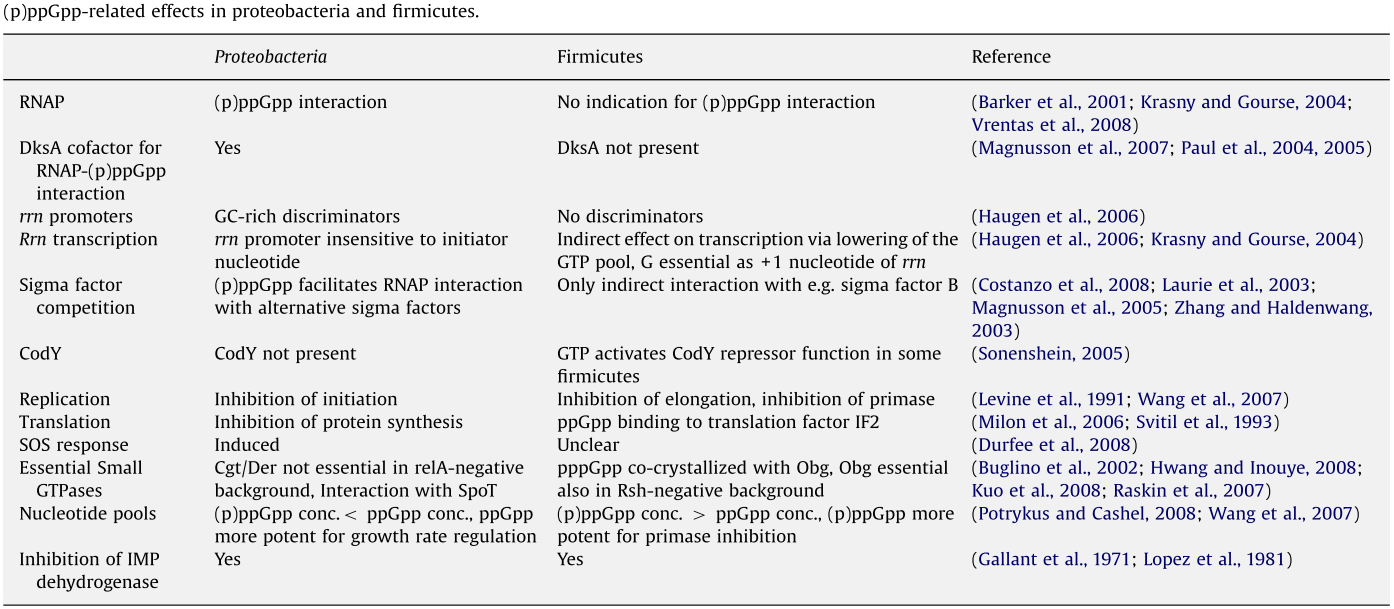
\includegraphics[width=17cm]{figure/compareStringentColiSubtilisTable.png}\\
  \caption{Comparison of stringent response between Escherichia Coli and Bacillus Subtilis \citep{wolz_synthesis_2010}}\label{tab:compareColiSubPhysiology}
\end{table}
More generally, it is suggested in \citep{kanjee_direct_2012} that the alarmones can bind in place of GTP in the three GTPase categories: translation co-factors (EF-G, EF-Tu, IF2), cell-signalling and cell-division (Obg) and protein translocation.

%\medskip

\paragraph{Alarmones effect on ATP and GTP pool in \textit{B. Subtilis}}
This effect is illustrated in Figure \ref{fig:alarmoneEnergyReg} and in more details in Figure \ref{fig:alarmoneGTPReg} for GTP.
\begin{figure}[hbtp]
  \centering
  % Requires \usepackage{graphicx}
  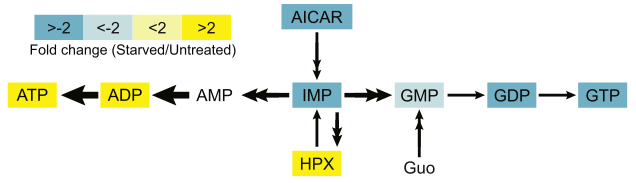
\includegraphics[width=15cm]{figure/alarmoneEnergy.png}\\
  \caption{Bacillus Subtilis: regulation of ATP and GTP pool by the alarmones \citep{kriel_direct_2012}}\label{fig:alarmoneEnergyReg}
\end{figure}
\begin{figure}[hbtp]
  \centering
  % Requires \usepackage{graphicx}
  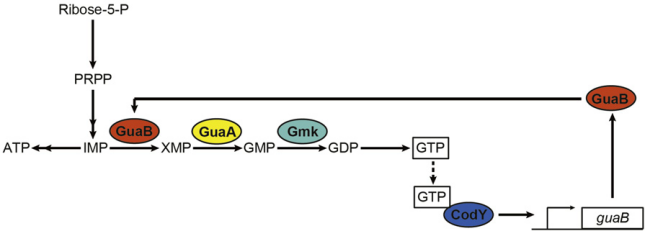
\includegraphics[width=10cm]{figure/alarmoneGTPPathway1.png} \\ 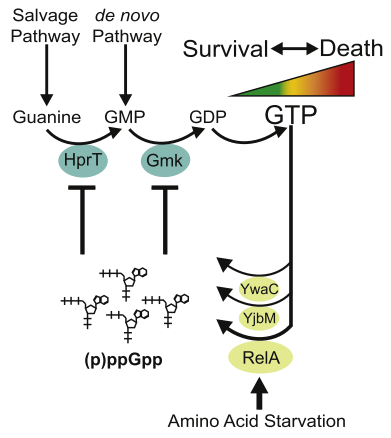
\includegraphics[width=6cm]{figure/alarmoneGTPPathway2.png}\\
  \caption{Bacillus Subtilis: GTP pathway regulation \citep{kriel_direct_2012}}\label{fig:alarmoneGTPReg}
\end{figure}
The regulation of GTP pool via the alarmones is more importantly performed by Gmk and HprT than by GuaB \citep{kriel_direct_2012}. The $IC_{50}$ are: $\approx 20 \mu M$ for Gmk, $\approx 11 \mu M$ for HprT and $\approx 0.3-0.5 mM$ for GuaB.



